\documentclass[11pt, english, twocolumn]{article}

\usepackage{hyperref}
\usepackage[eng]{felipito}
\usepackage{stfloats}
\usepackage{mathpazo}

\usepackage[margin=0.8in, left=0.7in, right=0.7in]{geometry}
\usepackage{caption}
\captionsetup[figure*]{position=bottom}
\floatname{algorithm}{Algorithm}

\graphicspath{{./Graphics/}}

% Colors
\definecolor{urlcolor}{rgb}{0,.145,.698}
\definecolor{linkcolor}{rgb}{.71,0.21,0.01}
\definecolor{citecolor}{rgb}{.12,.54,.11}


% Document title
\title{\bf Problem Set 2 \\ Statistics, Computation and
Applications\\[-1ex]}
\author{Felipe del Canto}
\date{October, 2021}
    
\hypersetup{
	breaklinks=true,  % so long urls are correctly broken across lines
    colorlinks=true,
    urlcolor=urlcolor,
    linkcolor=linkcolor,
    citecolor=citecolor,
}

\begin{document}
    
\maketitle
   
\begin{figure*}[b]
	\centering
	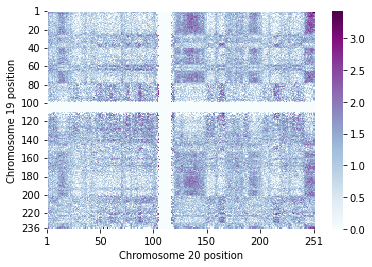
\includegraphics[width=0.4\textwidth]{19_20_heatmap}
	\caption{Heatmap for the average interaction between chromosomes 19 and 20. The values correspond to $\log(1 + \text{interaction frequency})$, darker colors represent a higher interaction frequency.}
	\label{fig:19-20-heatmap}
\end{figure*}

\section*{Problem 2.1}
For part (a), I first load the data and compute the mean ($\mu$) and standard deviation ($\sigma$) of $X := \log(1+ \texttt{interaction\_frequency})$, which are 1.13 and 0.40, respectively. Both numbers are rounded to the nearest hundredth. To compute these numbers, I use the fact that the sample variance ($\hat{\sigma}^{2}$) of data points $\{X_{1}, \ldots, X_{N}\}$ can be computed as
	$$\hat{\sigma}^{2} = \frac{1}{N}\sum_{i=1}^{N} X_{i}^{2} - \mu^{2}$$\\
where
	$$\mu = \frac{1}{N} \sum_{i=1}^{N} X_{i}$$ 
and compute, separately, the number of samples $N$, the sum of the squares of $X$ and the sum of $X$ by loading the datasets one at a time. Then, compute $\mu$ using the formula above and $\sigma = \sqrt{\hat{\sigma}^{2}}$.

For part (b), in \Cref{fig:19-20-heatmap} is presented the heatmap representing the interaction frequencies for chromosomes 19 and 20. As can be seen in the image, there are some contiguous darker zones that are indicators of intermingling portions of these chromosomes.

For part (c), we have that under the null hypothesis, $H_{0}$, the entries of the interaction matrix $M$ between any pair of chromosomes are independent and identically distributed according to a Normal distribution with mean $\mu$ and standard deviation $\sigma$. Consequently, given a $k \times \ell$ sub matrix of $M$, with mean $m$, we have that $m$ also follows a Normal distribution with mean $\mu$ but with standard deviation $\sigma/\sqrt{k\ell}$. Under the null, the probability of the $m$ being greater than $\mu$ is equal to
	\begin{equation} \label{eq:pvalueSubMatrix}
		1 - \Phi\left(\frac{m - \mu}{\sigma/\sqrt{k\ell}}\right)
	\end{equation}
This corresponds to the $p$-value of the test that rejects the null hypothesis of $\mu$ being the real mean, agains the alternative that the mean is lower. However, when looking for potential interaction zones (that is, submatrices with higher-than-average mean value), there are several hypothesis being tested at the same time. In fact, if $M$ is a $N_{r} \times N_{c}$ matrix, then for a fixed size of $k \times \ell$, there is a total of
	$$N_{\text{sumatrices}} := (N_{r} - k + 1)(N_{c} - \ell + 1)$$
possible submatrices of that size to test for interaction zones. Consequently, the $p$-value in (\ref{eq:pvalueSubMatrix}) must be adjusted for multiple testing hypothesis. In particular, if we follow the Bonferroni correction, the hypothesis is rejected (that is, we find interaction zones) at significance level $\alpha$ if
	$$1 - \Phi\left(\frac{m - \mu}{\sigma/\sqrt{k\ell}}\right) \leq \frac{\alpha}{N_{submatrices}},$$
which is what we wished to prove. In the case of the chromosomes 19-20 interaction matrix, we have that $M$ is of size $236 \times 251$ and if we wished to test for a $10 \times 10$ interaction region, we would have:
	$$N_{\text{submatrices}} = 54\,934$$
	
\begin{figure*}[t]
	\centering
	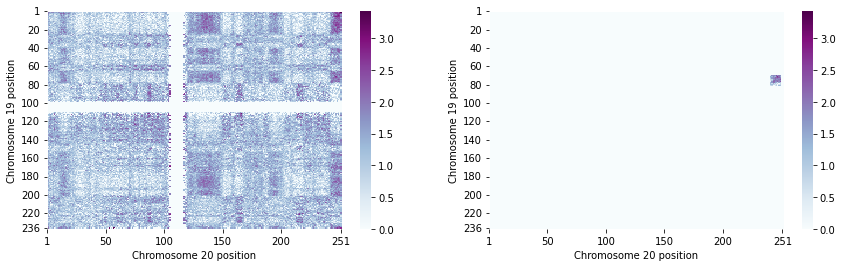
\includegraphics[width=.7\textwidth]{greedy-search}
	\caption{Greedy search algorithm finds an interaction region between chromosomes 19 and 20. To the left, the original interaction matrix. To the right, the submatrix found by the greedy search algorithm.}
	\label{fig:greedy-search}
\end{figure*}

\begin{figure*}[b]
	\centering
	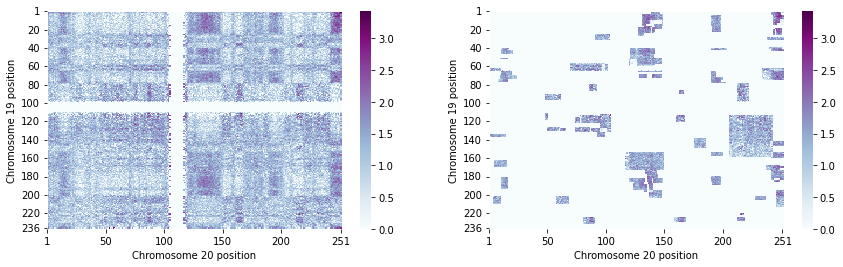
\includegraphics[width=.8\textwidth]{overall-greedy-search}
	\caption{Greedy search algorithm finds an interaction region between chromosomes 19 and 20. To the left, the original interaction matrix. To the right, the submatrix found by the greedy search algorithm.}
	\label{fig:overall-greedy-search}
\end{figure*}

For part (d), the greedy search algorithm is resumed in \Cref{alg:greedy-search}. This procedure works because, as the name suggests, greedily searches for submatrices whose mean is highly likely to be greater than $\mu$. This, because for any given initialization, the algorithm tries to find local minima in the adjusted $p$-value of each submatrix. To achieve this goal, when expanding the initial submatrix $M$ chooses the row or column that reduces the most the adjusted $p$-value. An example of how this algorithm finds an interacting region is presented in \Cref{fig:greedy-search}. As can be seen from the picture, the greedy search algorithm is capable of finding an interacting region. However, in order to find all possible interacting regions a more general purpose algorithm must be used. This new procedure is resumed in \Cref{alg:overall-greedy-search} and the result of running it for chromosomes 19 and 20 is presented in \Cref{fig:overall-greedy-search}. 


\begin{figure*}[t]
	\centering
	\begin{subfigure}{0.3\textwidth}
		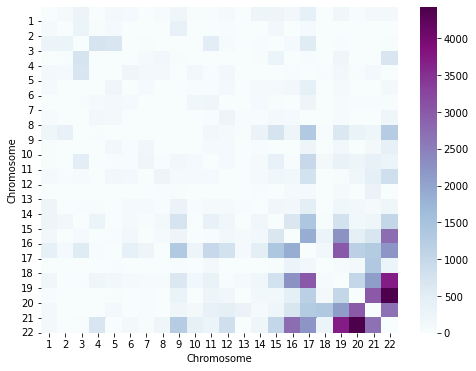
\includegraphics[width=\textwidth]{counting_regions}\\
		\caption{Heatmap of the number of intermingling regions for each pair of chromosomes.}
		\label{fig:counting-regions}
	\end{subfigure}\hfill
	\begin{subfigure}{0.3\textwidth}
		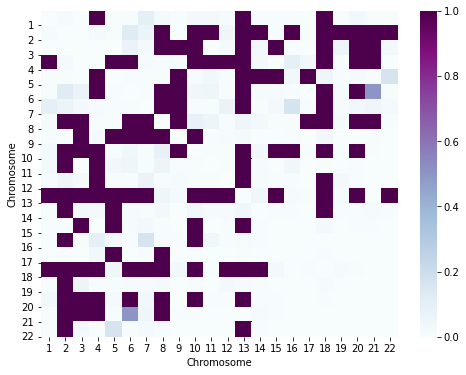
\includegraphics[width=\textwidth]{dissimilarity_matrix}\\
		\caption{Heatmap representing the dissimilarity matrix for each pair of chromosomes.}
		\label{fig:dissimilarity-matrix}
	\end{subfigure}
	\begin{subfigure}{0.3\textwidth}
		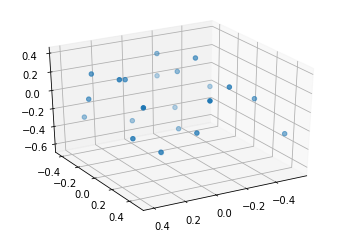
\includegraphics[width=\textwidth]{MDS_embedding}\\
		\caption{MDS embedding}
		\label{fig:MDS-embedding}
	\end{subfigure}
			\caption{3D embedding process for the chromosomes. In the left panel, the heatmap of the number of intermingling regions for each pair of chromosomes. In the center panel, the associated dissimilarity matrix. In the right panel, the MDS embedding is presented.}
\end{figure*}

For part (e), I first run \Cref{alg:overall-greedy-search} on all non equal pair of chromosomes to compute the number of intermingling regions. Since the goal is to embed these data into a 3D space, there is no need to compute these regions for identical chromosomes, as the distance between a chromosome and itself should be 0. The results are presented in \Cref{fig:counting-regions}. As can be seen from the image, some chromosomes have almost none interaction, while other share many regions. In particular, the most intermingled chromosomes are those at the lower right corner of the interaction counting matrix. These are the pairs: 16-22, 18-19, 19-20, 19-22, 20-21, 20-22, and 21-22.

\begin{algorithm}[H]
	\caption{Greedy search algorithm to the largest interaction region in interaction matrix $Z$}
	\label{alg:greedy-search}\vspace{1ex}
	\begin{algorithmic}
	\Function{greedy\_search}{\,\,}
		\State $M \gets \text{random } Z_{ij}$
		\State $p \gets $ adjusted $p$-value of $M$
		\State current\_$p$ $\gets p$
		\State return\_$M$ $\gets M$
		\While{$p \geq$  current\_$p$}
			\For{$side$ in [left, right, top, bottom]}
				\State $M_{2} \gets M$ + $side$ row/column
				\State $p_{2} \gets $ adjusted $p$-value of $M_{2}$
				\If{$p_{2}$ < current\_$p$}
					\State current\_$p$ $\gets p_{2}$
					\State return\_$M$ $\gets M_{2}$
				\EndIf
			\EndFor
		\EndWhile
		\State\Return return\_$M$
	\EndFunction
	\end{algorithmic}
\end{algorithm}

For part (f), in order to transform the count of intermingling region into a dissimilarity matrix that is accepted for the MDS algorithm, we need to transform the previous heatmap. This, in order to transform smaller (reps. large) counts into large (resp. smaller) distances. Let $D$ be the dissimilarity matrix that is wished to obtain. I first define that the diagonal of $D$ will contain only zeros, that is, each chromosome is identical to itself. Then, if the intermingling region count between chromosomes $i$ and $j$ is 0, then $D(i,j) = 1$. 

\begin{algorithm}[H]
	\caption{General procedure to find all interaction regions in an interaction matrix $Z$.}
	\label{alg:overall-greedy-search}\vspace{1ex}
	\begin{algorithmic}
	\Function{overall\_greedy\_search}{max\_rep}
		\State min\_$p$ $\gets$ 0.01
		\While{True}
			\For{$i$ in 1,$\ldots$,max\_rep}
				\State $M$ $\gets$ \Call{greedy\_search}{\,\,}
				\State $p_{2}$ $\gets$ adjusted $p$-value of $M$
				\If{$p_2 \leq$ min\_$p$}
					\State chosen\_$M$ $\gets$ $M$
					\State min\_$p$ $\gets$ $p_{2}$
				\EndIf
			\EndFor
			\If{min\_$p$ $\geq$ 0.01}
				\State break {\bf while}
			\EndIf
			\State $Z_{ij}$ $\gets$ $Z_{ij}$ - mean chosen\_$M$ 
		\EndWhile
		\State\Return return\_$M$
	\EndFunction
	\end{algorithmic}
\end{algorithm}

Finally, if the count is not zero, then $D(i,j)$ is equal to the inverse of the intermingling region count. This way, $D(i,j) \in [0,1]$ and lower values correspond to closer chromosomes. The final dissimilarity matrix is presented in \Cref{fig:dissimilarity-matrix}. As expected from \Cref{fig:counting-regions} and the definition of $D$, the heatmap shows a smaller distance for pairs of chromosomes whose interaction count was high and a distance close to 1 for those that had less (or none) interactions. Finally, using $D$ I perform the MDS embedding. The result is presented in \Cref{fig:MDS-embedding}.



\section*{Problem 2.2}

For part (a), note that duplicating the variable and running an \textit{unregularized} version of the logistic regression changes the output coefficient to $\frac{1}{2}\hat{\beta}$. Indeed, let $X' = 2X$ be the duplicated variable and let $h$ be the loss function for the logistic regression (which depends on the product $\beta Y$). Note that
	\begin{equation} \label{eq:dupX}
		\argmin_{\beta} h(\beta Y) = \frac{1}{2}\argmin_{\beta} h\left(\frac{1}{2}\beta Y\right).
	\end{equation}
Indeed, if $\beta^{*}$ solves the left-hand side problem, then $2\beta^{*}$ solves the right-hand one, and (\ref{eq:dupX}) is obtained. Hence,
	$$\argmin_{\beta} h(\beta Y) = \frac{1}{2}\argmin_{\beta}h(\beta X)$$
and the previous result is proved. Denoting $\beta^{*}$ the output coefficient obtained in the unregularized problem with $X$ doubled, we have that
	\begin{equation}\label{eq:ineq-betaHat}
		 \left|\beta^{*}\right| \leq \left|\hat{\beta}\right|,
	\end{equation}

with equality if and only if $\hat{\beta} = 0$. Finally, it should be expected that
	\begin{equation}\label{eq:ineq-betaL1}
		\left|\hat{\beta}_{\ell_{1}}\right| \leq \left|\beta^{*}\right|,
	\end{equation}
since the $\ell_{1}$-regularized problem induces a lower 1-norm for the output coefficient. To see why this happens, consider the regularized problem
	\begin{equation} \label{eq:l1-prob}
		\argmin_{\beta} h(\beta Y) + \lambda |\beta|.
	\end{equation}
for which $\beta^{*}$ is feasible and achieves the lowest $h$. Let $\hat{\beta}_{\ell_{1}}$ be the solution of (\ref{eq:l1-prob}). Then, $h\left(\hat{\beta}_{\ell_{1}}Y\right) \geq h\left(\beta^{*}Y\right)$. But since $\hat{\beta}_{\ell_{1}}$ is optimal, it has to occur that $\left|\hat{\beta}_{\ell_{1}}\right| \leq \left|\beta^{*}\right|$, otherwise $\beta^{*}$ would be the solution of (\ref{eq:l1-prob}).

In conclusion, we have that (\ref{eq:ineq-betaHat}) and (\ref{eq:ineq-betaL1}) imply
	$$\left|\hat{\beta}_{\ell_{1}}\right| \leq \left|\hat{\beta}\right|$$
with equality if and only if $\hat{\beta} = 0$, in which case $\hat{\beta}_{\ell_{1}} = 0$ as well.\\[1ex]

For part (b), we have that (\ref{eq:ineq-betaHat}) still holds. Moreover, the same argument use with optimization problem (\ref{eq:l1-prob}) holds with the $\ell_{2}$-regularized problem
	\begin{equation} \label{eq:l2-prob}
		\argmin_{\beta} h(\beta Y) + \lambda \beta^{2}.
	\end{equation}
and thus we have that
	\begin{equation}\label{eq:ineq-betaL2}
		\hat{\beta}_{\ell_{2}}^{2} \leq (\beta^{*})^{2},
	\end{equation}
but since $\hat{\beta}_{\ell_{2}}$ and $\beta^{*}$ are scalars, then (\ref{eq:ineq-betaL2}) is equivalent to (\ref{eq:ineq-betaL1}). Showing that
	$$\left|\hat{\beta}_{\ell_{2}}\right| \leq \left|\hat{\beta}\right|$$
with equality if and only if $\hat{\beta} = 0$, in which case $\hat{\beta}_{\ell_{2}} = 0$ as well.\\[1ex]

Finally, for part (c), one of the advantages of the elastic net is that, as opposed to $\ell_{1}$ regularization, there is always a unique solution. In situations with many features it might be the case that $\ell_{1}$ achieves two distinct and optimal results that are difficult to compare. If in that case the $\ell_{2}$ was used, many (if not all) features will have a nonzero coefficient, making the regularization less useful. Instead, by using the elastic net, it is possible to reduce de dimensionality of the coefficient vector while still ensuring a unique and tractable solution.

An example where the use of an elastic net could be beneficial would be a clinical application, where from the many risk factors only a few must be selected in order to provide physicians with a manageable tool to evaluate their patients. Another case would be selecting engineered features that can better explain a corpus when performing text classification. In order for results to be explainable and improved between training-testing iterations, a stable and interpretable solution must be obtained at each time.

\begin{figure*}[b]
	\centering
	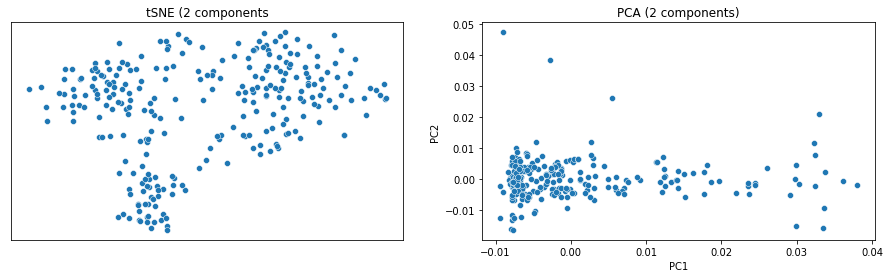
\includegraphics[width=0.8\textwidth]{tSNE-PCA}
	\caption{$t$-SNE (left) and PCA (right) plots for the sample of cells.}
	\label{fig:tSNE-PCA}
\end{figure*}

\section*{Problem 2.3}

For part (a), note that if $Y\,|\,X \sim \textrm{Bernoulli}\left(p(x)\right)$, then
	$$P(Y = y) = \left(1-p(x)\right)^{1-y}p(x)^{y}$$

Consequently, the likelihood of the $n$ iid observations is
	\begin{equation*} \resizebox{.45 \textwidth}{!}{
		$L\left( \{x_{i}, y_{i}\} ;\beta, \beta_{0}\right) 
		= \prod_{i=1}^{n} \left(1-p(x_{i}; \beta, \beta_{0})\right)^{1-y_{i}} p(x_{i}; \beta, \beta_{0})^{y_{i}},$
	}\end{equation*}
where
	$$p(x_{i}; \beta, \beta_{0}) = \frac{1}{1 + \exp\left(\beta_{0} + \beta^{T}x_{i}\right)}$$
And finally, the $\log$-likelihood is
	\begin{align*}
		\ell\left(\{x_{i}, y_{i}\}; \beta, \beta_{0}\right) 
			&=	\sum_{i=1}^{n} (1-y_{i})\log\left(1 - p(x_{i}; \beta, \beta_{0})\right) \\
			&\qquad\quad	+ y_{i}\log p(x_{i}; \beta, \beta_{0})
	\end{align*}
which after rearranging and canceling terms is
	\begin{align*}
		\ell\left(\{x_{i}\}; \beta, \beta_{0}\right) 
			&=	\sum_{i=1}^{n} (1-y_{i})\left(\beta_{0} + \beta^{T}x_{i}\right) \\
			&\qquad\quad	- \log\left(1+\exp\left(\beta_{0} + \beta^{T}x_{i}\right)\right)
	\end{align*}
And since the first term is nonzero only if $y_{i} = 0$, we can write
    \begin{align*}
		\ell\left(\{x_{i}, y_{i}\}; \beta, \beta_{0}\right) 
			&=	\sum_{\substack{i=1 \\ y_{i}=0}}^{n} \left(\beta_{0} + \beta^{T}x_{i}\right)	\\
			&\qquad	- \sum_{i=1}^{n}\log\left(1+\exp\left(\beta_{0} + \beta^{T}x_{i}\right)\right)
	\end{align*}

For part (b), let $\phi$ be the standard normal pdf. For $c \in \{0,1\}$, let
	$$z_{i,c} := -\frac{1}{2}(x_{i} - \mu_{c})^{T}\Sigma^{-1}(x_{i} - \mu_{c})$$

Then, following the same generalization for part (a), the likelihood for this $n$ iid observations is
	\begin{align*}
		L(\{x_{i}, y_{i}\}; \{\mu_{c}\}, \Sigma) =
			\prod_{i=1}^{n} \phi(z_{i,0})^{1-y_{i}} \phi(z_{i,1})^{y_{i}} 
	\end{align*}
And thus, the $log$-likelihood is
	\begin{align*}
		\ell(\{x_{i}, y_{i}\}; \{\mu_{c}\}, \Sigma) =
			\sum_{\substack{i=1 \\ y_{i} = 0}}^{n} \log \phi(z_{i,0}) + \sum_{\substack{i=1 \\ y_{i} = 1}}^{n} \log \phi(z_{i,1}) 
	\end{align*}
	
\section*{Problem 2.4}


\begin{figure*}[t]
	\centering
	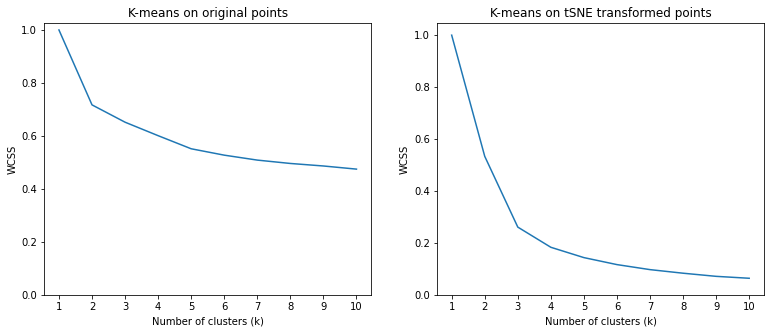
\includegraphics[width=0.7\textwidth]{fit-clusters}
	\caption{Within Cluster Sum of Squares (WCSS) for $k$-means algorithm ran with different number of clusters. The left (resp. right) image, shows WCSS for $k$-means applied on the original (resp. $t$-SNE transformed) data points.}
	\label{fig:fit-clusters}
\end{figure*}


For part (a), in order to choose the appropriate number of clusters ($k$), first we visualize the dataset to obtain a clue of how many groups of cells we could encounter. In \Cref{fig:tSNE-PCA} are presented the scatterplots that result of fitting a $t$-SNE and a PCA with two components each. In the left image, $t$-SNE hints at the possibility of three clusters, as the scatterplot shows a triangular shape. On the other hand, the image on the right suggests that PCA is not a good tool to search for clusters in this setting. Overall, I consider the possibility of up to 8 clusters. To test how many clusters is optimal in this case, in \Cref{fig:fit-clusters} is presented the Within Cluster Sum of Squares (WCSS) for different number of clusters, when running $k$-means for $k \in \{1,\ldots,k\}$ on both the original data points and the $t$-SNE transformed ones. In this figure, is possible to appreciate that applying $k$-means on the transformed points achieves a much better WCSS than when applied to the original data points. This is expected as $t$-SNE makes closer points appear closer, while increasing the distance between points that are separate beforehand. Looking at the image, it is possible to conclude that a number of clusters between 3 and 5 appears to be enough, as the elbow point in both images is between this range. 

In order to visualize how the clustering is being performed, in \Cref{fig:tSNE-clusters} are presented the scatterplots showing each of the clusters when applying $k$-means in the original and transformed data points. As can be seen in the pictures, the clusters formed when using $k$-means in the transformed data points are more structured than its counterparts to the left. For the rest of this problem, 4 clusters on the $t$-SNE transformed points were considered.

\begin{table*}[b]
	\caption{Relevant genomic features which predict the selected number of clusters. A Logit classifier was trained on the 4 labels (4 clusters) and the relevant genomic features and their values were extracted.}
	\label{tab:trapnell-logit}
	\begin{tabular}{ccccc}
		\hline\hline
		\\[-1.5ex]
		\multirow{2.5}{*}{Cluster}
					&&	\multicolumn{3}{c}{Relevant features}	\\[0.5ex]\cline{3-5}
					\\[-1.5ex]
					&&	Number		&	Position	&	Value	\\[0.5ex] \hline
		\\[-1.5ex]
		1			&&	1			&	13\,895		&	-\,0.32	\\[1ex]
		\multirow{2}{*}{2}
					&&	\multirow{2}{*}{2}
									&	13\,895		&	-\,0.04	\\
					&&				&	94\,839		&	\hspace{1ex}0.06	\\
		\\[-1.5ex]
		3			&&	1			&	13\,895		&	0.83	\\[1ex]
		4			&&	0			&	--			&	--		\\[0.5ex]
		\hline\hline
	\end{tabular}

\end{table*}

Finally, in order to find which genomic features are good markers for the 4 clusters selected, I train a classifier on the data. Specifically, a Logit model is trained to predict the labels of the 4 clusters using all features (RNA sequences) and regularizing using an elastic net. Since the data is extremely high-dimensional, the regularizing term allows for better interpretability of the results. Moreover, the elastic net also founds a unique solution no matter the initial conditions of the algorithm. The results are presented in \Cref{tab:trapnell-logit}. From what can be seen in the table, the sequence 13\,895 plays an important role in differentiating these cells. For example, cluster 1 is characterized by an under-regulation of sequence 13\,895, while cluster 3 is characterized by an over-regulation of the same sequence. Cluster 4, on the other hand is a type of cell that also has an under-regulation of sequence 13\,895, albeit in a smaller scale. However, it is also different from cluster 1 since this cell has an over-regulation of sequence 94\,839. Finally, cluster 4 has no relevant genomic features. In a not presented experiment, using 3 clusters leads to finding the same three relevant genomic features, suggesting cluster 4 is probably not a different cell type. 

\begin{figure*}[b]
	\centering
	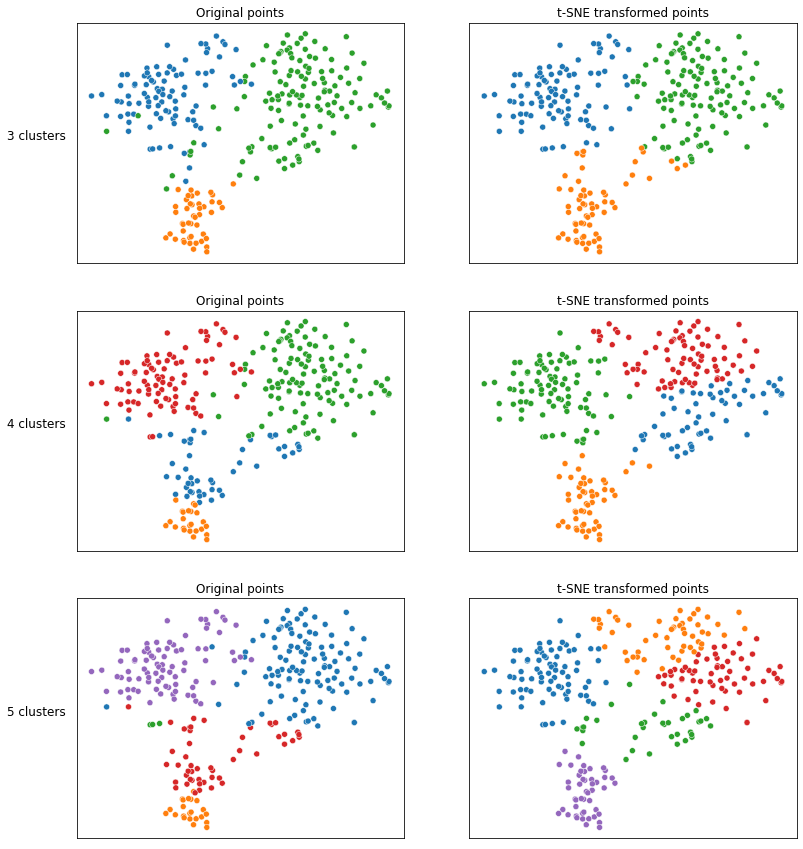
\includegraphics[width=\textwidth]{tSNE-clusters}
	\caption{$t$-SNE showing clustering of data points. The rows represent different number of clusters. The left (resp. right) column, shows the clustering when the $k$-means was applied on the original (resp. $t$-SNE transformed) data points.}
	\label{fig:tSNE-clusters}
\end{figure*}

  


\end{document}
